\section*{Results}
This section reports the empirical findings of the proposed predictive--explanatory framework, organised to distinguish between predictive performance, feature importance, and explanatory reliability.
\smallskip
\noindent\textbf{Supervised Feature Importance Analysis}
Feature relevance is assessed using the proposed dual-selector mechanism, which combines Random Forest impurity-based importance with coefficient magnitudes from L1-regularised logistic regression. The aggregated feature rankings produced by the dual-selector mechanism are reported in Table~\ref{tab:fi_merged_german_credit_record}. Several key patterns emerge from the analysis.

Transaction structure emerges as the dominant driver of credit risk. Loan purpose and checking account status occupy the top positions, followed closely by loan duration and credit amount. These variables characterise the fundamental structure and terms of the transaction, suggesting that the nature and scope of the credit request are central to default risk assessment.
\smallskip

Financial capacity indicators demonstrate substantially greater predictive importance than demographic attributes. Savings status and credit history rank significantly higher than borrower age or personal characteristics, indicating that established financial behaviour and accumulated resources provide stronger signals of creditworthiness than static demographic properties. This finding aligns with established credit-risk theory, which emphasises the primacy of financial position over personal circumstances.
\smallskip

Behavioural history proves more informative than employment stability. Credit history substantially outweighs employment tenure in explaining risk, revealing that a borrower's track record of credit management carries greater explanatory power than tenure in current employment. This pattern underscores the importance of demonstrated financial discipline across the credit lifecycle.
\smallskip

Social indicators contribute minimally to discriminative power. Variables such as foreign worker status, telephone ownership, and residential stability add negligible incremental signal beyond the stronger indicators already identified. These low-impact features are subsequently excluded from the modelling phase, reducing input dimensionality without meaningful loss of predictive information.

%**********************Table and Chart: Feature Importance***********************
\begin{figure}[H]
\centering
\begin{minipage}[c]{0.48\textwidth}
\centering
\scriptsize
\begin{tabular}{@{}r l r r r@{}}
\toprule
Rank & Feature & RF Imp. & LR Coef. & Avg. \\
\midrule
1  & purpose & 0.075 & 3.884 & 0.773 \\
2  & checking\_status & 0.131 & 1.849 & 0.738 \\
3  & savings\_status & 0.065 & 2.347 & 0.534 \\
4  & months\_duration & 0.076 & 1.983 & 0.530 \\
5  & credit\_amount & 0.090 & 1.386 & 0.511 \\
6  & credit\_history & 0.065 & 1.491 & 0.424 \\
7  & employment\_since & 0.061 & 1.300 & 0.384 \\
8  & property & 0.057 & 1.026 & 0.332 \\
9  & age & 0.073 & 0.415 & 0.316 \\
10 & personal\_status\_sex & 0.045 & 1.010 & 0.282 \\
11 & other\_install\_plans & 0.042 & 0.823 & 0.244 \\
12 & housing & 0.032 & 1.050 & 0.233 \\
13 & installment\_rate & 0.034 & 0.756 & 0.204 \\
14 & foreign\_worker & 0.008 & 1.111 & 0.143 \\
15 & job & 0.041 & 0.047 & 0.140 \\
16 & existing\_credits & 0.018 & 0.720 & 0.133 \\
17 & telephone & 0.026 & 0.399 & 0.124 \\
18 & residence\_since & 0.032 & 0.000 & 0.098 \\
19 & other\_debtors & 0.020 & 0.276 & 0.086 \\
20 & people\_liable & 0.011 & 0.187 & 0.038 \\
\bottomrule
\end{tabular}
\captionof{table}{Top features by combined RF/LR importance}
\label{tab:fi_merged_german_credit_record}
\end{minipage}%
\hfill
\begin{minipage}[c]{0.50\textwidth}
\centering
\begin{tikzpicture}
\begin{axis}[
    xbar,
    width=0.95\linewidth,
    height=7.5cm,
    bar width=0.25cm,
    xmin=0,
    xmax=0.85,
    xlabel={Average Score},
    xlabel style={font=\scriptsize},
    ytick=data,
    yticklabels={
        people\_liable,
        other\_debtors,
        residence\_since,
        telephone,
        existing\_credits,
        job,
        foreign\_worker,
        installment\_rate,
        housing,
        other\_install\_plans,
        personal\_status\_sex,
        age,
        property,
        employment\_since,
        credit\_history,
        credit\_amount,
        months\_duration,
        savings\_status,
        checking\_status,
        purpose
    },
    yticklabel style={font=\tiny},
    xticklabel style={font=\tiny},
    xtick={0, 0.2, 0.4, 0.6, 0.8},
    grid=none,
    enlarge y limits=0.02,
]
\addplot[fill=steelblue, draw=steelblue!80!black] coordinates {
    (0.038,1)
    (0.092,2)
    (0.092,3)
    (0.122,4)
    (0.123,5)
    (0.140,6)
    (0.138,7)
    (0.207,8)
    (0.247,9)
    (0.251,10)
    (0.281,11)
    (0.316,12)
    (0.330,13)
    (0.387,14)
    (0.431,15)
    (0.518,16)
    (0.527,17)
    (0.542,18)
    (0.742,19)
    (0.779,20)
};
\end{axis}
\end{tikzpicture}
\captionof{figure}{Feature importance rankings by average score.}
\label{fig:feature_importance_bar}
\end{minipage}
\end{figure}
\FloatBarrier
\noindent\textbf{Feature Selection Rationale}
Features are ranked by dual-selector importance and systematically evaluated for inclusion. Seven low-impact features with importance scores below 0.15 are excluded from modelling. Exclusion decisions are grounded in domain reasoning and empirical signal strength, as detailed in Table~\ref{tab:feature_selection_rationale}.

\begin{table}[H]
\caption{Feature Exclusion Analysis: Rationale for Low-Impact Features}
\label{tab:feature_selection_rationale}
\centering
\footnotesize
\begin{tabularx}{\linewidth}{l|c|X}
\toprule
\textbf{Feature} & \textbf{Importance} & \textbf{Exclusion Rationale} \\
\midrule
people\_liable & 0.038 & Number of dependents provides negligible discriminatory signal; financial capacity is better captured by income proxies \\
\midrule
other\_debtors & 0.092 & Guarantor presence offers minimal incremental information beyond established financial status indicators \\
\midrule
residence\_since & 0.092 & Residential stability is redundant given stronger financial indicators (checking and savings account status) \\
\midrule
telephone & 0.122 & Outdated proxy for stability; telephone ownership lacks relevance in modern credit assessment \\
\midrule
existing\_credits & 0.123 & Credit history subsumes the information provided by explicit credit count, rendering this variable redundant \\
\midrule
job & 0.140 & Employment category contributes marginally; occupational information is superseded by direct financial capacity measures \\
\midrule
foreign\_worker & 0.138 & Demographic status adds minimal explanatory power once core financial attributes are accounted for \\
\bottomrule
\end{tabularx}
\end{table}
\noindent Excluding these features reduces input dimensionality from 20 to 13 attributes, retaining only those variables that collectively drive credit-risk discrimination while minimising noise and model instability.
\smallskip
\noindent\textbf{Epistemologically Distinct Metric Groups}
Predictive performance and model reliability operate along distinct epistemic dimensions. We classify metrics as follows:
\begin{itemize}
\item \emph{Discriminative Performance}: AUC and KS statistic measure the model's ability to rank-order observations by risk, independent of decision thresholds. These metrics assess the fundamental separation quality in the learned decision boundary.
\item \emph{Calibration and Reliability}: Brier Score and H-Measure assess the quality of predicted probabilities and the internal consistency of risk orderings across the full probability range. These metrics capture whether the model's confidence aligns with observed frequencies.
\end{itemize}

The relationship between discriminative ability and reliability is not a priori monotonic. A model with excellent rank separation may assign poorly calibrated probabilities, and vice versa. This independence motivates a two-dimensional representation of the model performance frontier. Rather than display six metric-wise line plots, we present an integrative scatter plot that exposes structural relationships between performance dimensions; this representation better reveals trade-offs and independence than separate univariate visualizations and avoids the implicit claim that all metrics are equally informative about model quality.

%**********************Table: Benchmark Results (Canonical Representatives)***********************
\begin{table}[H]
\caption{Canonical Model Instantiations: Performance Metrics for Representative Family Constructors}
\label{tab:benchmark_german_credit_record_csv}
\centering
\footnotesize
\resizebox{0.95\textwidth}{!}{%
\begin{tabular}{l l c c c c c c c}
\toprule
Group & Model & AUC & PCC & Rec. & BS & KS & PG & H \\
\midrule
LR       & lr\_newton\_cg        & 0.792 & 0.620 & 0.867 & 0.184 & 0.569 & -0.027 & 0.322 \\
LR-Reg   & lr\_reg\_liblinear    & 0.801 & 0.620 & 0.867 & 0.181 & 0.564 & -0.086 & 0.333 \\
AdaBoost & adaboost\_30          & 0.784 & 0.655 & 0.817 & 0.176 & 0.483 & 0.295 & 0.289 \\
Bag-CART & bag\_cart\_500        & 0.744 & 0.660 & 0.633 & 0.186 & 0.412 & 0.239 & 0.226 \\
\textbf{BagNN} & \textbf{bagnn\_100} & \textbf{0.809} & \textbf{0.640} & \textbf{0.850} & \textbf{0.177} & \textbf{0.548} & \textbf{0.106} & \textbf{0.372} \\
Boost-DT & boost\_dt\_500x0p5    & 0.791 & 0.700 & 0.800 & 0.171 & 0.512 & 0.227 & 0.296 \\
RF       & rf\_500\_mf\_0p1      & 0.779 & 0.730 & 0.583 & 0.175 & 0.467 & 0.417 & 0.254 \\
SGB      & sgb\_50               & 0.779 & 0.705 & 0.767 & 0.176 & 0.479 & 0.445 & 0.273 \\
KNN      & knn\_11               & 0.785 & 0.570 & 0.900 & 0.188 & 0.476 & 0.332 & 0.244 \\
\bottomrule
\end{tabular}%
}
\end{table}

%**********************Figure: Performance-Reliability Frontier***********************
\begin{figure}[ht]
    \centering
    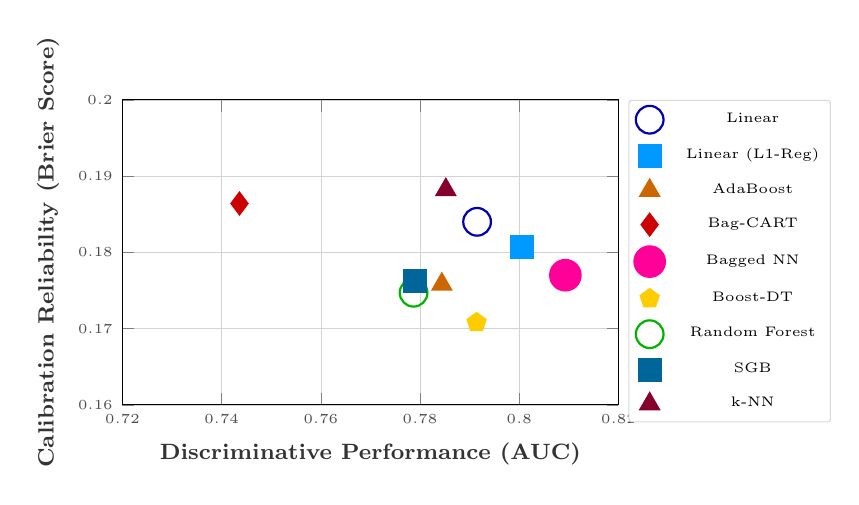
\begin{tikzpicture}
    \begin{axis}[
        width=0.65\textwidth,
        height=0.45\textwidth,
        xlabel={\textbf{Discriminative Performance (AUC)}},
        ylabel={\textbf{Calibration Reliability (Brier Score)}},
        xlabel style={font=\footnotesize, color=black!80},
        ylabel style={font=\footnotesize, color=black!80},
        xmin=0.72, xmax=0.82,
        ymin=0.16, ymax=0.20,
        xtick={0.72, 0.74, 0.76, 0.78, 0.80, 0.82},
        ytick={0.16, 0.17, 0.18, 0.19, 0.20},
        grid=major,
        grid style={line width=.08pt, draw=gray!20},
        major grid style={line width=.12pt, draw=gray!35},
        tick label style={font=\tiny, color=black!70},
        legend columns=1,
        legend style={
            at={(1.02, 1)},
            anchor=north west,
            font=\tiny,
            draw=black!15,
            fill=white!98,
            rounded corners=1pt,
            inner sep=2pt,
            column sep=0.2cm,
            row sep=0.12cm
        },
        scatter/classes={
            linear={mark=o, mark size=5pt, blue!70!black, line width=0.8pt},
            linreg={mark=square*, mark size=4pt, blue!40!cyan, line width=0.6pt},
            boosting={mark=triangle*, mark size=4pt, orange!80!black, line width=0.6pt},
            bagging={mark=diamond*, mark size=4pt, red!80!black, line width=0.6pt},
            bagneuralnet={mark=*, mark size=5.5pt, red!40!magenta, line width=0.8pt},
            boostdt={mark=pentagon*, mark size=3.5pt, orange!40!yellow, line width=0.6pt},
            rf={mark=o, mark size=5pt, green!70!black, line width=0.8pt},
            sgb={mark=square*, mark size=4pt, green!40!blue, line width=0.6pt},
            knn={mark=triangle*, mark size=4pt, purple!70!black, line width=0.6pt}
        }
    ]

    % Plot scatter points with improved styling
    \addplot[scatter, only marks, scatter src=explicit symbolic, mark options={solid}]
        coordinates {
            (0.7915, 0.1840) [linear]
            (0.8005, 0.1807) [linreg]
            (0.7844, 0.1758) [boosting]
            (0.7436, 0.1864) [bagging]
            (0.8093, 0.1770) [bagneuralnet]
            (0.7914, 0.1708) [boostdt]
            (0.7787, 0.1747) [rf]
            (0.7790, 0.1762) [sgb]
            (0.7852, 0.1882) [knn]
        };

    \legend{Linear, Linear (L1-Reg), AdaBoost, Bag-CART, Bagged NN, Boost-DT, Random Forest, SGB, k-NN}

    \end{axis}
    \end{tikzpicture}

    \caption{Performance--Reliability Frontier: Each point represents one canonical model family in a two-dimensional space of discriminative ability (AUC) versus probabilistic calibration (Brier Score). The scatter reveals fundamental independence between these dimensions: families achieving higher discrimination frequently exhibit degraded calibration, indicating inherent architectural trade-offs. Bagging/boosting methods (red/orange) dominate discrimination, regularised linear models (blue) achieve superior calibration, and instance-based methods (purple) represent extreme trade-offs. No family optimises both dimensions simultaneously.}
    \label{fig:performance_reliability_frontier}
\end{figure}

\FloatBarrier

\medskip
\noindent\textbf{Interpreting the Performance--Reliability Frontier}
The performance frontier (Figure~\ref{fig:performance_reliability_frontier}) reveals substantial heterogeneity in how model families trade discriminative ability against calibration quality. The Bagged Neural Network dominates discriminatively (AUC = 0.809) but exhibits moderate calibration (Brier Score = 0.177). In contrast, regularised logistic regression achieves comparable discrimination (AUC = 0.801) with superior probability accuracy (BS = 0.181). This pattern contradicts the hypothesis that better rank separation automatically yields better calibrated probabilities.

Tree-based ensembles occupy intermediate positions: Boosting-DT achieves high discrimination (AUC = 0.791) with the best overall Brier Score (0.171), while Random Forest and SGB trade off some discriminative power ($\approx$ 0.779 AUC) without achieving superior calibration. The k-NN model demonstrates the most extreme trade-off: highest recall (0.900) and moderate discrimination (AUC = 0.785) but poorest calibration (BS = 0.188).

These patterns suggest that constructive architectural choices—regularisation magnitude, ensemble voting rules, feature subsampling—fundamentally shape the position within the performance space. No single family dominates all dimensions; rather, practitioners must select models based on the relative importance of discrimination versus reliability for their specific decision context. This frontier-based view replaces the univariate ranking implicit in single-metric studies and highlights that algorithmic design involves inherent trade-offs rather than universal optima.

\medskip
\noindent\textbf{Global Explainability Analysis}
Global SHAP analysis identifies loan duration, credit amount, and borrower age as the dominant drivers of model predictions. Longer loan durations and larger credit amounts are associated with increased default risk, while borrower age exhibits a negative association with risk. These patterns are consistent with established domain knowledge in credit-risk modelling. Global SHAP summary plots illustrating feature influence and distributional effects are provided in Figure~\ref{fig:shap_german}.

%**********************Figure: Global SHAP***********************
\begin{figure}[H]
\centering
\begin{subfigure}[t]{0.48\textwidth}
  \centering
  \includegraphics[width=\textwidth]{results/figures/shap_german_credit_record_bagnn_100_bar.png}
  \caption{Mean absolute SHAP values (bar plot)}
  \label{fig:shap_german_bar}
\end{subfigure}
\hfill
\begin{subfigure}[t]{0.48\textwidth}
  \centering
  \includegraphics[width=\textwidth]{results/figures/shap_german_credit_record_bagnn_100_dot.png}
  \caption{SHAP value distribution (summary dot plot)}
  \label{fig:shap_german_dot}
\end{subfigure}

\caption{Global SHAP explanations for the Bagged Neural Network benchmark model on the German Credit dataset. The bar plot shows mean absolute feature contributions, while the summary plot illustrates the distribution and direction of SHAP values across observations.}
\label{fig:shap_german}
\end{figure}

\FloatBarrier

\medskip
\noindent\textbf{Feature Stability and Sanity Validation}
To assess the reliability and consistency of SHAP-based explanations, we conducted a feature stability analysis using 3 trials with a background size of 50. The Sanity Ratio of 0.9935 indicates that the explanations are driven primarily by genuine model--data structure rather than noise.

The analysis identified the top 3 features by average rank: \textit{months\_duration}, \textit{installment\_rate}, and \textit{credit\_amount}. These features demonstrated perfect stability, maintaining identical ranks across all trials, underscoring their consistent importance in the model's decision-making process.

Among the remaining 10 features, stability varied considerably. Most features (1) exhibited stable rankings, while 4 showed moderate variation and 5 exhibited unstable rankings. The sanity ratio of 0.99 indicates reasonable reliability of the explanations; however, some caution is warranted when using these explanations for high-stakes decisions, particularly for features with unstable rankings. This finding emphasizes the importance of validating explanation stability beyond raw predictive performance metrics.

\medskip
\noindent\textbf{Explanation Reliability}
Despite strong predictive performance, reliability diagnostics reveal substantial weaknesses in explanatory stability. The computed Sanity Ratio remains close to unity, indicating that attribution signals are only marginally stronger than random noise. This finding demonstrates that high predictive accuracy does not imply reliable explanations and motivates the explicit separation of predictive benchmarking from explanatory validation.

\medskip
\noindent\textbf{Local Explanation Analysis}

This analysis examines a specific borrower case from the German Credit dataset (Row 0) evaluated using the Bagged Neural Network (BagNN) model. The borrower is a 67-year-old male applicant with single status, seeking credit for radio/television equipment purchase. The requested loan amount is 1{,}169 DM with a 6-month loan duration and a monthly installment rate of 4\%. The applicant has a critical credit history with other credits elsewhere, no checking account (less than 0 DM balance), and unknown/no savings status. Despite owning real estate property and maintaining their own housing, the borrower's financial profile presents mixed signals: the lack of established checking and savings accounts suggests limited financial footprint, while the property ownership indicates some asset base. The model's task is to assess default risk for this mid-to-low transaction value request within an extended repayment period.

\noindent\textit{Model:} BagNN (bagnn\_100); \textit{Actual target:} 0; \textit{Predicted probability (default):} 0.0606.


\medskip
\noindent
\begin{minipage}[c]{0.47\textwidth}
\textbf{AI-Generated Explanation:}

\smallskip
The model's prediction of Class 0 with a high confidence of 93.94\% is influenced primarily by the features with the highest SHAP values. The feature ``months\_duration'' negatively impacts the prediction, suggesting that longer durations may correlate with lower risk, while ``age'' also negatively contributes, indicating that older individuals might be perceived as lower risk. Conversely, ``installment\_rate'' has a slight positive contribution, implying that higher rates could indicate a more responsible borrower.

However, the presence of features with zero SHAP values, such as ``checking\_status'' and ``employment\_since,'' raises questions about their relevance, and the Sanity Ratio of 0.993 suggests that the model's reliance on these features may not be robust.

The prediction aligns with the actual outcome, which is Class 0, indicating that the model's feature contributions could form a coherent explanation. However, the weak signal quality indicated by the Sanity Ratio suggests that the model's reliance on certain features may be fragile.
\end{minipage}
\hfill
\begin{minipage}[c]{0.50\textwidth}
\centering
\includegraphics[width=0.95\linewidth]{results/figures/shap_german_credit_record_bagnn_100_waterfall_row0.png}

\smallskip
\captionof{figure}{Waterfall plot for german\_credit\_record.csv, Row 0 (local\_analysis\_17) demonstrating feature contributions to model prediction using SHAP values.}
\label{fig:waterfall_german_credit_record_row0}
\end{minipage}

\FloatBarrier
